% Diese Zeile bitte -nicht- aendern.
\documentclass[course=erap]{aspdoc}
%%
\newcommand{\theGroup}{196} 
\newcommand{\theNumber}{A328} 
\author{⁨Aleksandre Kandelaki \and Matthias Staritz \and Benjamin Liertz}
\date{Sommersemester 2020/21} 
%%
% Diese Zeile bitte -nicht- aendern.
\title{Gruppe \theGroup{} -- Abgabe zu Aufgabe \theNumber}
\usepackage{gauss}
\begin{document}
\maketitle

%%%%%%%%%%%%%%% Einleitung %%%%%%%%%%%%%%%%%%
\section{Einleitung}
Im Folgenden wird im Rahmen einer Projektarbeit im Fach Einführung
in die Rechnerarchitektur an der TU München ein in der linearen Algebra häufig 
benutztes Verfahren genauer beschrieben, implementiert und enstprechend dokumentiert.\\

Das Verfahren LU-Zerlegung, auch LR-Zerlegung genannt,
bietet eine Möglichkeit per Algorithmus lineare Gleichungssysteme zu lösen und Matrixinverse zu bestimmen. 
Dies Findet z.B. Anwendung bei der Berechnung des Stromflusses in Schaltkreisen. Mit der LU-Zerlegung kann man, 
wenn man die Wiederstände einzelner Leitungen gegeben hat, den Stromfluss an jedem Wiederstand berechnen. \cite{LUAnwendung}
Dazu liefert die LU-Zerlegung für jedes eindeutig lösbare Gleichungssystem $A \cdotx = b$, also wenn $A$ regulär ist,
zwei Dreiecksmatrizen $L$ und $U$ und eine Pivot-Matrix $P$,
wobei $P \cdot L \cdot U = A$ ergibt. Hierbei haben die Matrizen besondere 
Eigenschaften. $L$ hat in allen Einträgen oberhalb der Diagonalen die Werte 0 (siehe Matrix \ref{unteremx}). 
$U$ hingegen hat in allen Einträgen unterhalb der Diagonalen die Werte 0 (siehe Matrix \ref{oberemx}). 
Die Matrix $P$ ist eine Einheitsmatrix mit ggf. vertauschten Zeilen.\\\\
%%%%%%% (1) %%%%%%%%%
  \begin{equation}
    Untere \, Dreiecksmatrix : \begin{bmatrix}
    \caption{\label{unteremx}}
    l_{1,1}    & 0        &  0       & \cdots   & 0\\
    l_{2,1}    & l_{2,2}  &  0	      &          & \vdots\\
    l_{3,1}	& l_{3,2}  & l_{3,3}  & \ddots   & \vdots\\
    \vdots	    & \vdots   & \vdots   & \ddots   & 0 \\
    l_{n,1}	& l_{n,2}  & l_{n,3}  & \cdots   & l_{n, n} \\
    \end{bmatrix}
  \end{equation}\\\\

%%%%%%% (2) %%%%%%%%%
  \begin{equation}
    Obere \, Dreiecksmatrix: \begin{bmatrix}
    \caption{\label{oberemx}}
    u_{1,1} & u_{1,2} & u_{1,3}  & \cdots & u_{1,n} \\
    0	     & u_{2,2} & u_{2,3}  & \cdots & u_{2,n}\\
    0	     & 0       & u_{3,3}  & \cdots & u_{3,n}\\
    \vdots  & \vdots  &          & \ddots & \vdots\\
    0       & 0       & \cdots   & 0      & u_{n, n}\\
    \end{bmatrix}
  \end{equation}
  \\

Ein anschauliches Beispiel hierzu wäre das lineare Gleichungssystem:
%%%%%%% (3-6) %%%%%%%%%
  \begin{eqnarray}
    0x_1 + 3x_2 + 5x_3 + 7x_4 = 0 \\
    2x_1 + 6x_2 + 10x_3 + 14x_4 = 0\\
    -4x_1 + 12x_2 + 15x_3 + -21x_4 = 0\\
    6x_1 + 9x_2 + -5x_3 + -7x_4 = 0
  \end{eqnarray}

Welches auch durch folgende Koeffizientenmatrix dargestellt werden kann:
%%%%%%% (7) %%%%%%%%%
  \begin{equation}
    A = \begin{bmatrix}
    0	& 3	 & 5  & 7 \\
    2	& 6	 & 10 & 14 \\
    -4	& 12 & 15 & -21\\
    6	& 9  & -5 & -7\\
    \end{bmatrix}
  \end{equation}

Nach Anwendung der LU-Zerlegung ergeben sich folgende Matrizen:
%%%%%%% (8) %%%%%%%%%
  \begin{equation}
    A = \begin{bmatrix}
    0	& 3	 & 5  & 7 \\
    2	& 6	 & 10 & 14 \\
    -4	& 12 & 15 & -21\\
    6	& 9  & -5 & -7\\
    \end{bmatrix}
    L =
    \begin{bmatrix}
    1	& 0	 & 0  & 0 \\
    0	& 1	 & 0 & 0 \\
    -2	& 8 & 1 & 0\\
    3	& -3  & 4 & 1\\
    \end{bmatrix}
    U =
    \begin{bmatrix}
    2	& 6	 & 10 & 14 \\
    0	& 3	 & 5 &  7 \\
    0	& 0  & -5 & -49\\
    0	& 0  & 0 &  168\\
    \end{bmatrix}
    P =
    \begin{bmatrix}
    0	& 1	 & 0 & 0 \\
    1	& 0	 & 0 & 0 \\
    0	& 0  & 1 & 0\\
    0	& 0  & 0 & 1\\
    \end{bmatrix}
  \end{equation}
 
 
%%%%%%%%%%%%%%% Lösungsansatz %%%%%%%%%%%%%%%%%%

\section{Lösungsansatz}
Zur Durchführung dieser Zerlegung haben wir uns entschieden ein Programm auf Basis des gaußschen Eliminationsverfahren zu enwickeln.
Das gaußsche Eliminationsverfahren ändert die Einträge einer Matrix unter Verwendung elementarer Zeilenoperationen.
Die verwendeten elementaren Zeilenoperationen sind das Tauschen zweier Zeilen (siehe Gleichung \ref{swap}) und 
das Addieren von Vielfachen einer Zeile auf eine Andere (Siehe Gleichung \ref{add}). 
Dabei wird das Gleichungssystem $A \cdot x = b$ verändert, die Lösung bleibt aber erhalten.\\

Mit diesem Verfahren wird die bereits genannte obere Dreiecksmatrix U generiert. So erhalten wir unsere $U$ Matrix. 
Um nun auch die Matrizen $L$ und $P$ zu erhalten, müssen wir nur alle Schritte die zur Generierung 
der $U$ Matrix beigetragen haben dokumentieren. Jedes mal, wenn wir eine Zeile auf eine Andere addieren,
wird dies in der $L$ Matrix festgehalten, indem genau dieselbe Operation auf dieser $L$ Matrix durchgeführt wird. 
Jede Zeilenvertauschung wird auf die selbe Art in $P$ festgehalten.  Um nun sicher eine gültige $L$ Matrix zu erhalten, 
welche oberhalb der Diagonalen nur die 0 als Einträge hat und somit die gesuchte untere Dreiecksmatrix bildet, 
folgt der Algorithmus strikt der Vorgehensweise des Gauß Algorithmus.\\

Gehen wir davon aus, dass wir für jede der Matrizen $L$, $U$ und $P$ einen Speicherplatz vorhanden ist.
Dann müssen zu Beginn die für den Algorithmus notwendigen Startwerte dort abgelegt werden. Für $L$ und $P$ sind das 
reguläre Einheitsmatrizen, während in $U$ zu Beginn die Eingabematrix $A$ gespeichert wird. Nun werden die Einträge unterhalb 
der Diagonalen in $U$ spaltenweise von links nach rechts auf 0 gesetzt indem man immer ein genau passendes vielfaches 
einer oberen Zeile von allen darunterliegenden Zeilen abzieht. Die Wahl der Zeile hängt davon ab, welche Spalte gerade 
auf 0 gesetzt werden soll. Bei Spalte 1 ist es Zeile 1 bei Spalte 2 Zeile 2 und so weiter. Da man sich hierbei von oben 
nach unten bwz. von links nach rechts vorarbeitet generiert man schrittweise die gewünschten $L$ und $U$ Matrizen. 
Nun kann es aber vorkommen, dass in der Zeile welche von den anderen Zeilen subtrahiert werden soll an dem Index 
der zu bearbeitenden Spalte eine 0 steht. Dies birgt das Problem, dass nun kein vielfaches dieser Zeile jemals 
die anderen Einträge der Spalte durch Subtraktion auf 0 bringen kann, da $ 0 \times x = 0$. Um dieses Problem zu vermeiden 
haben wir uns entschieden unabhängig von der Eingabe, bevor wir mit der Nullung einer Zeile beginnen, immer die Zeile mit dem betragsmäßig größsten Eintrag
am entsprechenden Index nach oben zu tauschen (siehe Grafik). Dadurch wird garantiert, dass der Algorithmus bei einer 
regulären, quadratischen Matrix erfolgreich durchläuft. Im Abschnitt zur Genauigkeit wird noch genau darauf 
eingegeangen, warum wir immer die Zeile mit dem größten Eintrag nach oben tauschen und nicht bloß irgendeine Zeile 
mit Eintrag ungleich 0. Zusätzlich sei gesagt, dass nicht jede Matrixzerlegung den Schritt der Zeilenvertauschung 
benötigt und, dass der Algorithmus auf diese Art oft unnötige Vertauschungen durchführt was potential für 
Optimierungen bieten könnte.\\
 
Hier ein Beispiel für Zeilenvertauschungen:
  \begin{equation}
    \caption{\label{swap}}
    \centering
    \begin{gmatrix}[b]
    0	& 3	 & 5  & 7 \\
    2	& 6	 & 10 & 14 \\
    -4	& 12 & 15 & -21\\
    6	& 9  & -3 & -9
    \rowops 
    \swap{0}{3}
    \end{gmatrix}
    \rightarrow 
    \begin{gmatrix}[b]
    6	& 9  & -3 & -9\\
    2	& 6	 & 10 & 14 \\
    -4	& 12 & 15 & -21\\
    0	& 3	 & 5  & 7
    \end{gmatrix}
  \end{equation}\\

Hier ein Beispiel für Zeilenaddition:
  \begin{equation}
    \caption{\label{add}}
    \centering
    \begin{gmatrix}[b]

    6	& 9  & -3 & -9\\
    2	& 6	 & 10 & 14 \\
    -4	& 12 & 15 & -21\\
    0	& 3	 & 5  & 7

    \rowops 
    \add[\frac{1}{3}]{0}{2}
    \end{gmatrix}
    \rightarrow 
    \begin{gmatrix}[b]
    6	& 9  & -3 & -9\\
    2	& 6	 & 10 & 14 \\
    0	& 15 & 14 & -24\\
    0	& 3	 & 5  & 7
    \end{gmatrix}
  \end{equation}\\
 

\subsection{Stack vs. Heap}
Bei der Wahl des Speicherortes muss noch eine weitere Gegebenheit beachtet werden
und zwar haben wir hier die Wahl zwischen dem Heap und dem Stack. Aufgrund der besseren Zugriffszeiten würden wir den 
Stack als Speicherort präferieren, jedoch werden bei Linux-Betriebssystemen meistens nur ca. 8MB Speicherplatz für die 
Stackallokation zur Verfügung gestellt\cite{stack}\cite{stackSize}.Dies birgt das Problem, dass es bei großen Matrizen 
zu einem Segmentation Fault kommen kann, sofern der Stack als Speicher verwendet wird. Um trozdem die bessere 
Performance des Stacks nutzen zu können, haben wir eine Fallunterscheidung implementiert, welche je nach Größe der Matrix 
die Zerlegung auf dem Stack zerlegt oder den Speicherplatz auf dem Heap alloziiert. Die Maximalgröße einer Eingabematrix, 
deren Zerlegung auf dem Stack durchgeführt werden kann, berechnen wir folgender maßen: 
Die Größe der Eingabematrix $A$ muss 4 mal alloziert werden, da temporär $A$, $L$, $U$ 
und $P$ abgespeichert werdem müssen. Der in der Methode übergebene Parameter $n$ gibt die Anzahl Zeilen / Spalten der 
Matrix an, da unsere Matrizen immer quadratisch sein müssen. Dadurch ergibt sich eine Anzahl Einträge pro Matrix von $n \cdot n $. 
Jeder dieser Einträge ist in unserem Fall ein Floating Point Wert und somit 4 Bytes groß. Daraus ergibt sich die Formel 
\ref{size}, welche die benötigte Anzahl Bytes in Abhängigkeit unserer Eingabegröße $n$ berechnet.\\
  \begin{equation}
    \label{size}
    #bytes = 4 \cdot 4 \cdot n \cdot n
  \end{equation}
  Damit folgt, dass für eine Nutzung des Stacks $n \leq 707$ sein muss (\ref{maxsize}).
  \begin{equation}
    \label{maxsize}
    4 \cdot 4 \cdot n \cdot n \leq 8 \cdot 10^6
  \end{equation}
 Um etwas Spielraum zu haben haben wir uns entschieden schon ab einem $n \geq 700$ auf dem Heap zu allozieren.\\

\subsection{Verschiedene Implementierungen}
Wie eben schon erwähnt ist uns aufgefallen, dass die LU Zerlegung vieler Matrizen auch noch gelöst werden kann wenn man 
die Pivotisierung weg lässt. In der Theorie könnte man dadurch einen Performancegewinn erzielen. Um dies zu überprüfen, 
haben wir eine Vergleichsimplementierung erstellt, welche Pivotisierungen nicht berücksichtigt. Diese kann dann zwar nicht 
mehr jede Matrix zerlegen, ist aber potentiell schneller. Ansonsten ist diese Implementierung analog zu obigen Ansatz.\\ 
Den Ansatz mit Pivotisierung haben wir auf 4 verschiedene Arten umgesetzt. Einmal als einfaches, lineares C Programm 
und einmal als C Programm unter Verwendung von Intrinsics. Ebenso haben wir zwei verschiedene Assembler Implementierungen 
geschaffen. Wieder eine lineare Implementierung und eine Vektorisierte Version mit Hilfe von SIMD Operationen.
Auf die speziefischen Unterschiede wird im Abschnitt \ref{Performanzanalyse} noch genauer eingegangen.



%%%%%%%%%%%%%%% Genauigkeit %%%%%%%%%%%%%%%%%%

\section{Genauigkeit}
In diesen Abschnitt wird die Genauigkeit unserer Implementierung der LU-Zerlegung analysiert und anhand 
passender Beispiele demonstriert und getestet. Wir haben uns für die 
Genauigkeitsanalyse entschieden, da diese ein großes Problem bei der LU-Zerlegung 
darstellt, besonders wenn der Algorithmus ohne Pivotisierung arbeitet. In diesen Fall 
handelt es sich um einen instabilen Algorithmus und es kann zu komplett 
falschen Ergebnissen kommen. Das Problem der Genauigkeit ist auf die Kondition der 
Matrix A und auf die endliche Rechengenauigkeit von Computern zurückzuführen. \\

Im folgenden arbeiten wir mit Floats. Floats sind Gleitkommazahlen mit einer Größe 
bzw. Genauigkeit von 32 Bit und können neben einem sehr großen Wertebereich auch 
sehr genau Zahlen darstellen. Dies wird durch eine flexible Position des Kommas erreicht. 
Dennoch ist die Genauigkeit der Gleitkommazahlen allein durch die Endlichkeit an 
Rechenleistung und Speicher begrenzt. Somit beträgt die 
Genauigkeit im Folgenden immer ungefähr 8 Stellen. Aber auch bei Zahlen wie 
0,2 kommt es schon zu Rundungsfehlern, da diese in Gleitkommadarstellung im Binärsystem unendlich 
viele Stellen benötigen würde. Beim Darstellen von Zahlen als Gleitkommazahlen im Computer 
kommt es allgemein immer zu Störungen. So also auch in unserem Programm. z.B. beim Einlesen von A.\\
Neben den Darstellungsproblemen treten beim Rechnen mit Zahlen in Gleitkommadarstellung aber auch 
die Probleme der Absorption und Auslöschung auf, welche noch sehr viel größere Störungen bewirken können.

Problematisch wird dies, weil in der LU-Zerlegung $\frac{n^2}{2} - \frac{n}{2} $
Additionen und genau so viele Multiplikationen auftreten\cite{LUGenauigkeit}.
Durch die Gleitkommadarstellung kommt es nun also bei der LU-Zerlegung immer und 
unvermeidlich zu einer Vielzahl an Rundungsfehlern. Diese führen zu Störungen im Gleichungssystem $Ax=b$. 
In wie fern diese Störungen der Eingabedateien auch die Lösung des Problems stören, nennt man Kondition. 
Die Frage ist nun ob das Gleichungssystem gut oder schlecht konditioniert ist?

Hierzu ein Beispiel:
%%%%%%% (13) %%%%%%%%%
  \begin{equation}
    \label{absBeis}
    \begin{bmatrix}
    1	& 1	 \\
    1	& 1-\epsilon\\
    \end{bmatrix}
    \cdot x = 
    \begin{bmatrix}
    4 \\
    4- \epsilon\\
    \end{bmatrix}
    = b\;\;\;\;\;
    x = 
    \begin{bmatrix}
    3 \\
    1\\
    \end{bmatrix}
  \end{equation}

Störung der rechten Seite mit $ 0 < \epsilon \ll 1$:
%%%%%%% (14) %%%%%%%%%
  \begin{equation}
    \label{absBeis2}
    \bar{b} = b + 
    \begin{bmatrix}
    \epsilon \\
    -\epsilon\\
    \end{bmatrix}
    = \begin{bmatrix}
    4 + \epsilon\\
    4- 2\epsilon\\
    \end{bmatrix}
    \;\;\;\;\;
    \bar{x} = 
    \begin{bmatrix}
    1 + \epsilon \\
    3\\
    \end{bmatrix}
  \end{equation}

Hier lässt sich sehen, dass eine kleine Störung in $b$ dazu führen kann, 
dass das Gleichungssystem eine stark abweichende Lösung hat.
Dieses lineares Gleichungssystem ist also schlecht konditioniert. In der LU-Zerlegung stellt dies nun ein großes 
Problem dar, da hier durch die Rundungsfehler einige Störungen in Matrix $A$ auftreten.

Um zu verstehen, wie und ob die LU-Zerlegung verbessert werden kann, muss man 
zuerst das Problem weiter analysieren und verstehen, wie die Lösung des linearen 
Gleichungssystem von Störungen der Eingabe abhängt. 
Um die Größe einer Störung und die Abhängigkeit der Lösung von der Störung messen zu 
können, braucht man ein Maß. Hierfür bietet sich das Konzept der Normen an. Es wird aber 
auch die Norm für Matrizen benötigt, diese nennt man die zugehörige Matrizen Norm, 
welche wie folgt definiert ist: \\
es sei $||.||$ eine beliebige Norm auf $R^n$ dann ist  
%%%%%%% (15) %%%%%%%%% (Matrix-Norm)
  \begin{equation}
    \label{norm}
    ||A|| := sup_{x\neq 0}\;\frac{||Ax||}{||x||}\; \forall\; A \;\epsilon \;\mathbb{R}^{n \times n}
  \end{equation}

wodurch dann $||Ax||$ wie folgt abgeschätzt werden kann
  \begin{equation}
    \label{norm}
    ||Ax|| \leq ||A|| \cdot ||x||\;  \forall\; x \;\epsilon \;\mathbb{R}^n 
  \end{equation}

Mit dieser Definition einer Norm lässt sich nun die Kondition eines linearen 
Gleichungssystems genauer untersuchen. Sei $Ax=b$ unser lineares Gleichungssystem, 
welches leicht in b gestört wird, sodass nun $A \bar{x}=\bar{b}$ gilt.
Der rellative Fehler zur Größe $x$ entspricht also 
$\frac{||x-\bar{x}|}{||x||}$ und die relative Störung 
$\frac{||(b-\bar{b})||}{||b||}$. Dadurch ergibt sich nun 
%%%%%%% (17) %%%%%%%%% (relativer Fehler)
  \begin{equation}
    \label{norm}
    \frac{||x- \bar{x}||}{||x||}   \leq    \frac{||b||} {||x||} \cdot ||A^{-1}|| \cdot \frac{||b-\bar{b}||}{||b||} \leq ||A|| \cdot ||A^{-1}|| \cdot \frac{||(b-\bar{b})||} {||b||}
  \end{equation}
 
Hier definiert man nun $||A|| \cdot ||A^{-1}||$ als Kondition von $A$. Anders gesagt wird 
der relative Fehler durch die Kondition von $A$ mal der relativen Störung 
von oben beschränkt. Daraus lässt sich schließen, dass wenn die relative Störung klein 
ist, der relative Fehler nicht auch zwingend klein ist, sondern nur dann, wenn die 
Kondition von $A$ auch klein ist.
Jetzt haben wir aber nur $b$ gestört, wenn man nun auch die Matrix $A$ stört, dann ist 
unser gestörtes System nun $\bar{A} \bar{x} = \bar{b}$. Für dieses gilt nun folgender Satz, 
wenn $ea \cdot cond(A) < 1$ und $\frac{||A - \bar{A}||} {||A||} \leq ea $	und 	$\frac{||b - \bar{b}||} {||b||} \leq eb $, wobei 
$ea$ und $eb$ hier den Störungen in $A$ und $b$ entsprechen, ist:\\
%%%%%%% (18) %%%%%%%%%
  \begin{equation}
    \frac{||x-\bar{x}||} {||x||} \leq \frac{cond(A)} {1- ea \cdot cond(A)} \cdot (ea + eb)   
  \end{equation}
Es ist nun also sicher zu sagen, dass bei einer kleinen relativen Störung des linearen 
Gleichungssystems, auch die Kondition von $A$ klein sein muss, damit der relative Fehler 
klein bleibt, aber auch dass ein gewisser relativer Fehler unvermeidbar ist.

Die Frage ist nun, ob die LU-Zerlegung stabil ist.
Stabil ist ein Algorithmus, wenn er bei der Störung der Eingabedaten nur einen relativen Fehler macht, 
der in der selben Größenordnung liegt wie der unvermeidbare relative Fehler des Problems an sich. 
Allgemein heißt ein Algorithmus stabil im Sinne der Rückwärtsanalyse, 
falls $\hat{x}$ die exakte Lösung von $\hat{A}x = b$ ist mit 	
%%%%%%% (19) %%%%%%%%% (Stabilität)				
  \begin{equation}
    \label{norm}
    \frac{|| A - \bar{A}||}{||A||} \leq C \; eps \;\; \;\;\;\;\;\;\;\;  \frac{|| b - \bar{b}||}{||b||} \leq C \; eps
  \end{equation}

mit einem nicht all zu großem $C$, wobei $eps$ für die Maschinengenauigkeit steht.
Die LU-Zerlegung ermittelt nun, selbst wenn die Eingabe ohne Rundungsfehler erfolgt, $\hat{L}$ und $\hat{U}$ mit 
$\hat{x}$ als Ergebnis, da Rundungsfehler bei dem Verfahren auftreten. $\hat{x}$ ist dann die 
korrekte Lösung des linearen Gleichungssystems $\bar{A}x=b$ mit Störung in $\bar{A}$ bei der folgende Ungleichung gilt:
  \begin{equation}
    \label{eg3}
    |A - \bar{A}| \leq 2n \; eps \; |\bar{L}||\bar{R}| + O(eps^2)
  \end{equation}

Hierbei sind die Beträge und das $\leq$ komponentenweise zu verstehen.								
Nun wird ersichtlich, dass der Abstand zwischen $A$ und $\bar{A}$ auch von $|\hat{L}| \cdot |\hat{U}|$
abhängt. Dies wird problematisch, da der relative Abstand von $A$ zu $\bar{A}$ eigentlich durch 
$C\cdot eps$ abgeschätzt werden sollte. $|\hat{L}|$ und $|\hat{U}|$ lässt sich jedoch nicht sinnvoll 
beschränken, weshalb $C$ hier auch sehr groß werden kann.
Folglich ist die LU-Zerlegung ohne Spaltenpivotwahl instabil. Es lässt sich jedoch durch die Spaltenpivotisierung 
der Faktor $|\hat{L}|$  begrenzen. Dies liegt daran, dass nun für alle $i,j = 0,...,n |I_{i,j}| \leq 1$ gilt. 
Bei $|\hat{U}|$ lässt sich weiterhin keine gute Abschätzung finden und so gilt nun folgende Ungleichung:  
%%%%%%% (21) %%%%%%%%%
  \begin{equation}
    \label{eg3}
    \frac{||A - \bar{A}||\infty}{||A||\infty} \leq 2n^3 \; eps \;\frac{max_{i,j}| \hat{u}_{ij}|}{max_{i,j}|a_{ij}|} + O(eps^2)
  \end{equation}

Hier ist nun der Quotient das Problem bzw. entscheidet über die Stabilität der LU-
Zerlegung. Für diesen kann jedoch nur: $\frac{max_{i,j}| \hat{u}_{ij}|}{max_{i,j}|a_{ij}|} \leq 2^{n-1}$ angenommen 
werden, folglich ist der Algorithmus auch durch die Spaltenpivotwahl über die Menge 
aller invertierbaren Matrizen nicht stabil. Da sich der Quotient in der Realität mit zufälligen Matrizen deutlich 
besser abschätzen lässt, gilt die LU-Zerlegung mit Pivotsuche als stabil.



%%%%%%%%%%%%%%% Performanzanalyse %%%%%%%%%%%%%%%%%%

\section{Performanzanalyse}
\label{Performanzanalyse}
Die Laufzeit berechnet sich über  $ \frac{1}{3}n^3 -\frac{1}{3} n $ und befindet sich somit in $O(n^3)$ \cite{LULaufzeit}
In unserer Performanceanalyse vergleichen wir folgende Implementierungen:\\
\begin{itemize}
\item Lineare C Implementierung ohne Compileroptimierung und mit Pivotisierung vs. Lineare C implementierung ohne Compileroptimierung und ohne Pivotisierung. 
\item Lineare C Implementierung ohne Compileroptimierung vs. C Implementierung mit Vektorisierung durch Intrinsics. 
\item Lineare C Implementierung mit Compileroptimierung -O3 vs. Assembler Implementierung mit SIMD Vektorisierung.
\end{itemize}
Die Ergebnisse der Vergleiche werden in den folgenden Unterkapiteln ausgeführt. \\


\subsection{Pivotisierung vs. keine Pivotisierung}
Leider ist der Perfomace Gewinn wie man an Grafik \ref{PvsNP} unschwer erkennen kann wenn überhaut bloß maginal. Und dass obwohl wir zum Erstellen der Grafik mit Worst-case Eingaben gearbeitet haben bei denen $n-1$ mal pivotisiert werden musste.
Dies kann man vermutlich auf zwei grundlegende Effekte zurückführen. Erstens Verändert das weglassen der Pivotisierung nicht die
asymptotische Laufzeit welche weiterhin in $O(n^3)$ liegt. Der einzige Gewinn ligt also darin dass pro Schleifendurchlauf etwas weniger Operationen ausgeführt werden müssen. Dies kann aber maximal einen linearen Speedup erbringen. 
Dieser lineare Speedup ist aber ebenfalls nicht wirklich signifikant da, wie man mit einer Performance Analyse erkennt, die Pivotisierung so oder so nur einen sehr kleinen Prozentsatz der Laufzeit beansprucht. 
  \begin{figure}[H]
  \begin{center}
  \caption{Pivotisierend vs. Nicht-Pivotisierend} 
  \label{PvsNP}
  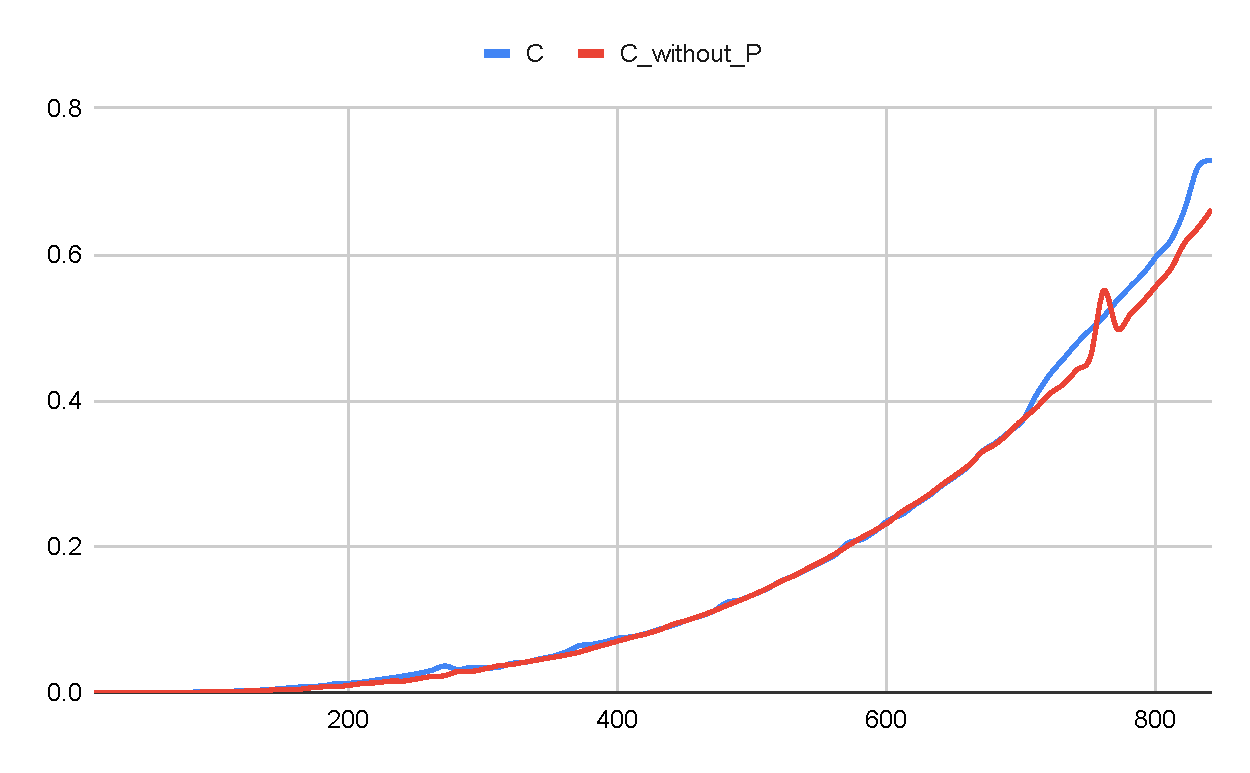
\includegraphics[width = 0.8\linewidth]{PvsNP.pdf}
  \end{center}
  \end{figure}
Unter Betrachtung dieser Erkenntnis zusätzlich zu den Ergebnissen der Genauigkeitsanalyse sind wir zu dem Schluss gekommen das eine Implementierung ohne Pivotisierung keinen Vorteil und Signifikante Nachteile bringt und dieser
Ansatz somit nicht weiter Verfolgt werden muss.

\subsection{Linear vs. Parallel durch Intrinsics}
Eine Performanzanalyse unserer Linearen C Implementierung mit perf tool hat ergeben, dass ein Großteil der Rechenzeit in einer bestimmten Schleife verbracht wird. Ausserdem zeigt perf tool uns, dass innerhalb der
Schleife die meiste Zeit für \textbf{mov} Befehle aufgewandt wird dicht gefolgt von arithmetischen Operationen. Diese Befehle sind in unserem Kontext Teil von Zeilenoperationen auf eine Matrix. Dies bedeutet,dass diese Operationen zu 
großen Teilen Unabhänig voneinander sind. Also können wir diese Operationen relativ einfach, unter Zuhilfenahme von C Intrinsics, parallelisieren.
Die Laufzeit der Implementierung in der wir diese teuren Operationen vektorisiert haben wird In Abbildung \ref{CvsIntrins} mit der Laufzeit der unvektorisierten Implementierung verglichen. \\
Durch den zusätzlichen Overhead der Vektorisieung sieht man bei kleineren Eingabegrößen keinen signifikanten Unterschied. Aber um so größer die Eingabe wird desto deutlicher sieht man, an den sich von einander entfernenden 
Graphen, dass die Vektorisierung einen guten Speedup generiert. 
Wir haben den Speedup Punktuell bei einer Eingabegröße von $n = 1000$ berechnet wo dieser bei $\approx 1.5$  liegt.\\
  \begin{figure}[H]
  \begin{center}
  \caption{C-linear vs. C-vektorisiert}
  \label{CvsIntrins}
  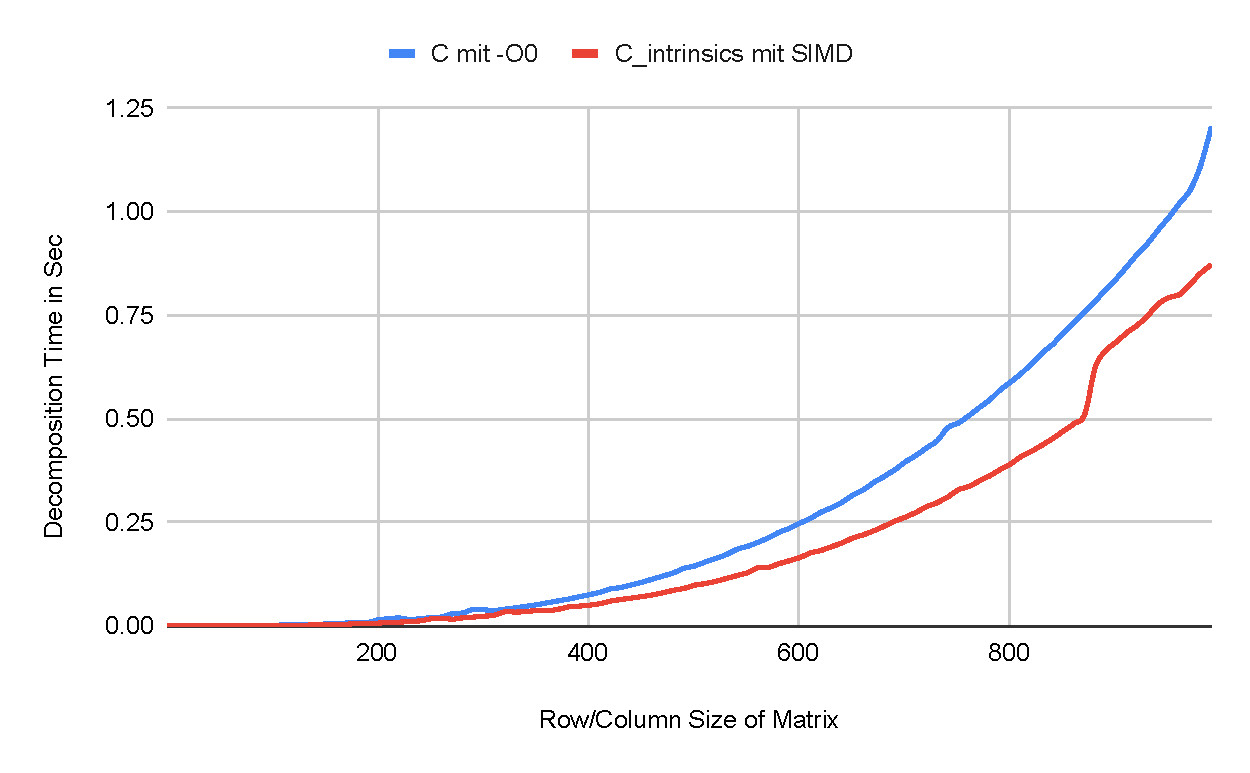
\includegraphics[width = 0.8\linewidth]{CvsIntrins.pdf}
  \end{center}
  \end{figure}

\subsection{Compiler optimierter Code vs. ASM mit SIMD}
Als letztes haben wir um optimale Performance zu erreichen eine reine ASM Implementierung entwickelt. In dieser Implementierung haben wir möglichst viel Optimiert und vor allem die im vorherigen Kapitel als Laufzeit aufwendig
intendefizierten Stellen direkt mit xmm Instruktionen Vektorisiert. Zum Vergleich haben wir unsere einfache C Implementierung mit -O3 kompilliert um zu analysieren ob unsere Implementierung besser, schlechter oder ähnlich gut wie der Compiler ist.
Wie man an Abbildung \ref{CvsASM} erkennen kann bringt unsere händische Implementierung eine deutlich bessere Performance als die compileroptimierte Version. Dies Ist ein für uns überraschendes Ergebnis was uns aber zeigt das 
es manchmal tatsächlich noch sinnvoll sein kann Assembler Code per Hand zu schreiben.
  \begin{figure}[H]
  \begin{center}
  \caption{Compileroptimiert vs. ASM-vektorisiert} 
  \label{CvsASM}
  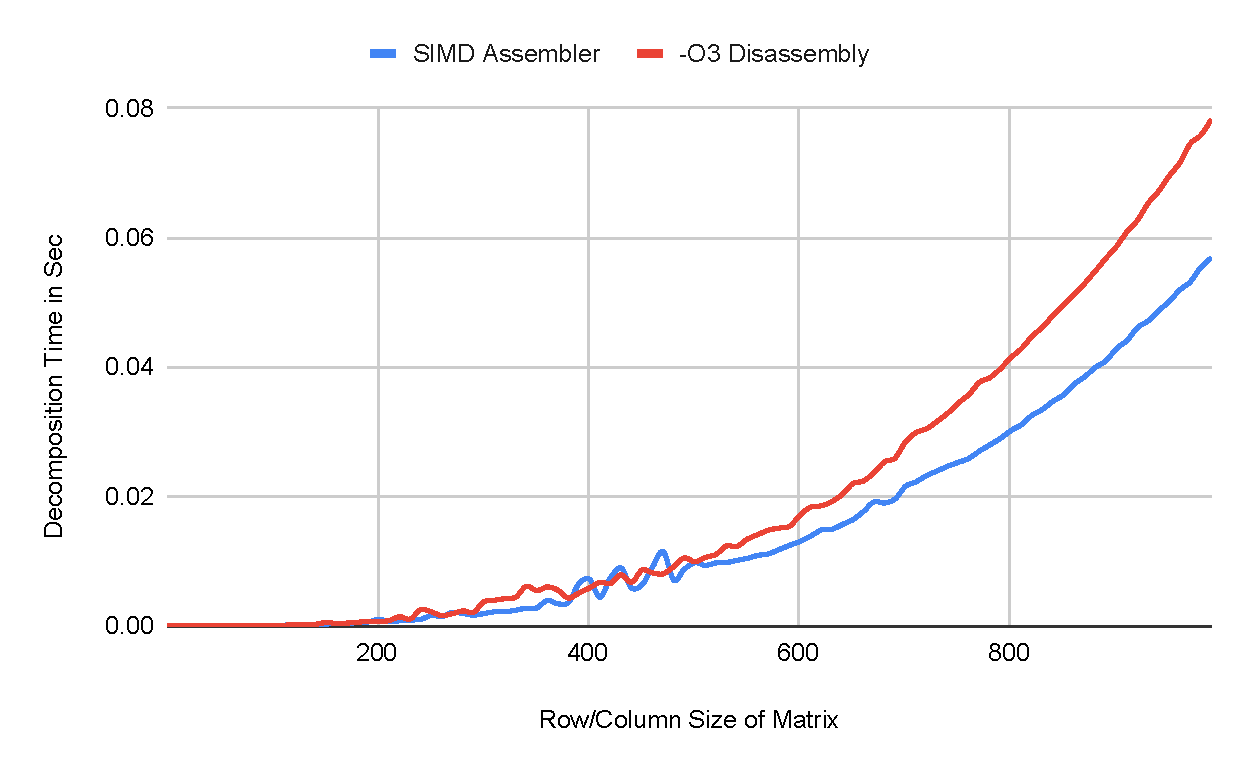
\includegraphics[width = 0.8\linewidth]{CvsASM.pdf}
  \end{center}
  \end{figure}



%%%%%%%%%%%%%%% Zusammenfassung %%%%%%%%%%%%%%%%%%

\section{Zusammenfassung und Ausblick}
Im laufe diser Ausarbeitung haben wir Verschiedee Implementiuerungen der LU Zerlegung Erstellt und miteinander verglichen. Es hat sich herrausgestellt dass Implementierungen ohne Pivotisierungen nicht zu Empfehlen sind,
die sie aufgrund von Floating-point arithmethischen Gegebenheitenheiten sehr ungenau sind und auch keinen sonderlichen Performance Gewinn erbringen. Performance techicht haben wir herrausgefunden dass eine per Hand vektorisierte ASM Implementierung am 
schnellsten läuft. Dies war für uns ein überraschendes ergebnis ,da wir davon ausgegangen sind, dass Compileroptimierter Code effizienter laufen würde.   
Welche Performance war jetzt am besten?\\
Rückblickend hätte man ohne pivotisierung weglassen können\\
% TODO: Fuegen Sie Ihre Quellen der Datei Ausarbeitung.bib hi
% Referenzieren Sie diese dann mit \cite{
% Beispiel: CR2 ist ein Register der x86-Architektur~\cite{intel2017man}.
\bibliographystyle{plain}
\bibliography{Ausarbeitung}{}

\end{document}

